
\documentclass[reprint,aps,prd,showpacs,nofootinbib]{revtex4-2}
\usepackage{graphicx,amsmath,amssymb}
\begin{document}
\title{A testable brane-world unification: rho$^2$ cosmology, dark radiation, and a GW spectral break}
\author{Ricardo Maldonado}
\affiliation{Independent Researcher}
\begin{abstract}
We present a minimal brane-world framework with a modified Friedmann equation
$H^2=\frac{8\pi G}3\rho\left(1+\frac{\rho}{2\lambda}\right)+\frac{\Lambda_4}3+\frac{\mathcal C}{a^4}$.
A single scale $\lambda$ controls a GW spectral break $f_{\rm br}\propto \lambda^{1/4}$ and a dark-radiation term linked to $\Delta N_{\rm eff}$.
\end{abstract}
\maketitle
\section{Data-anchored pass}
\begin{figure}[t]
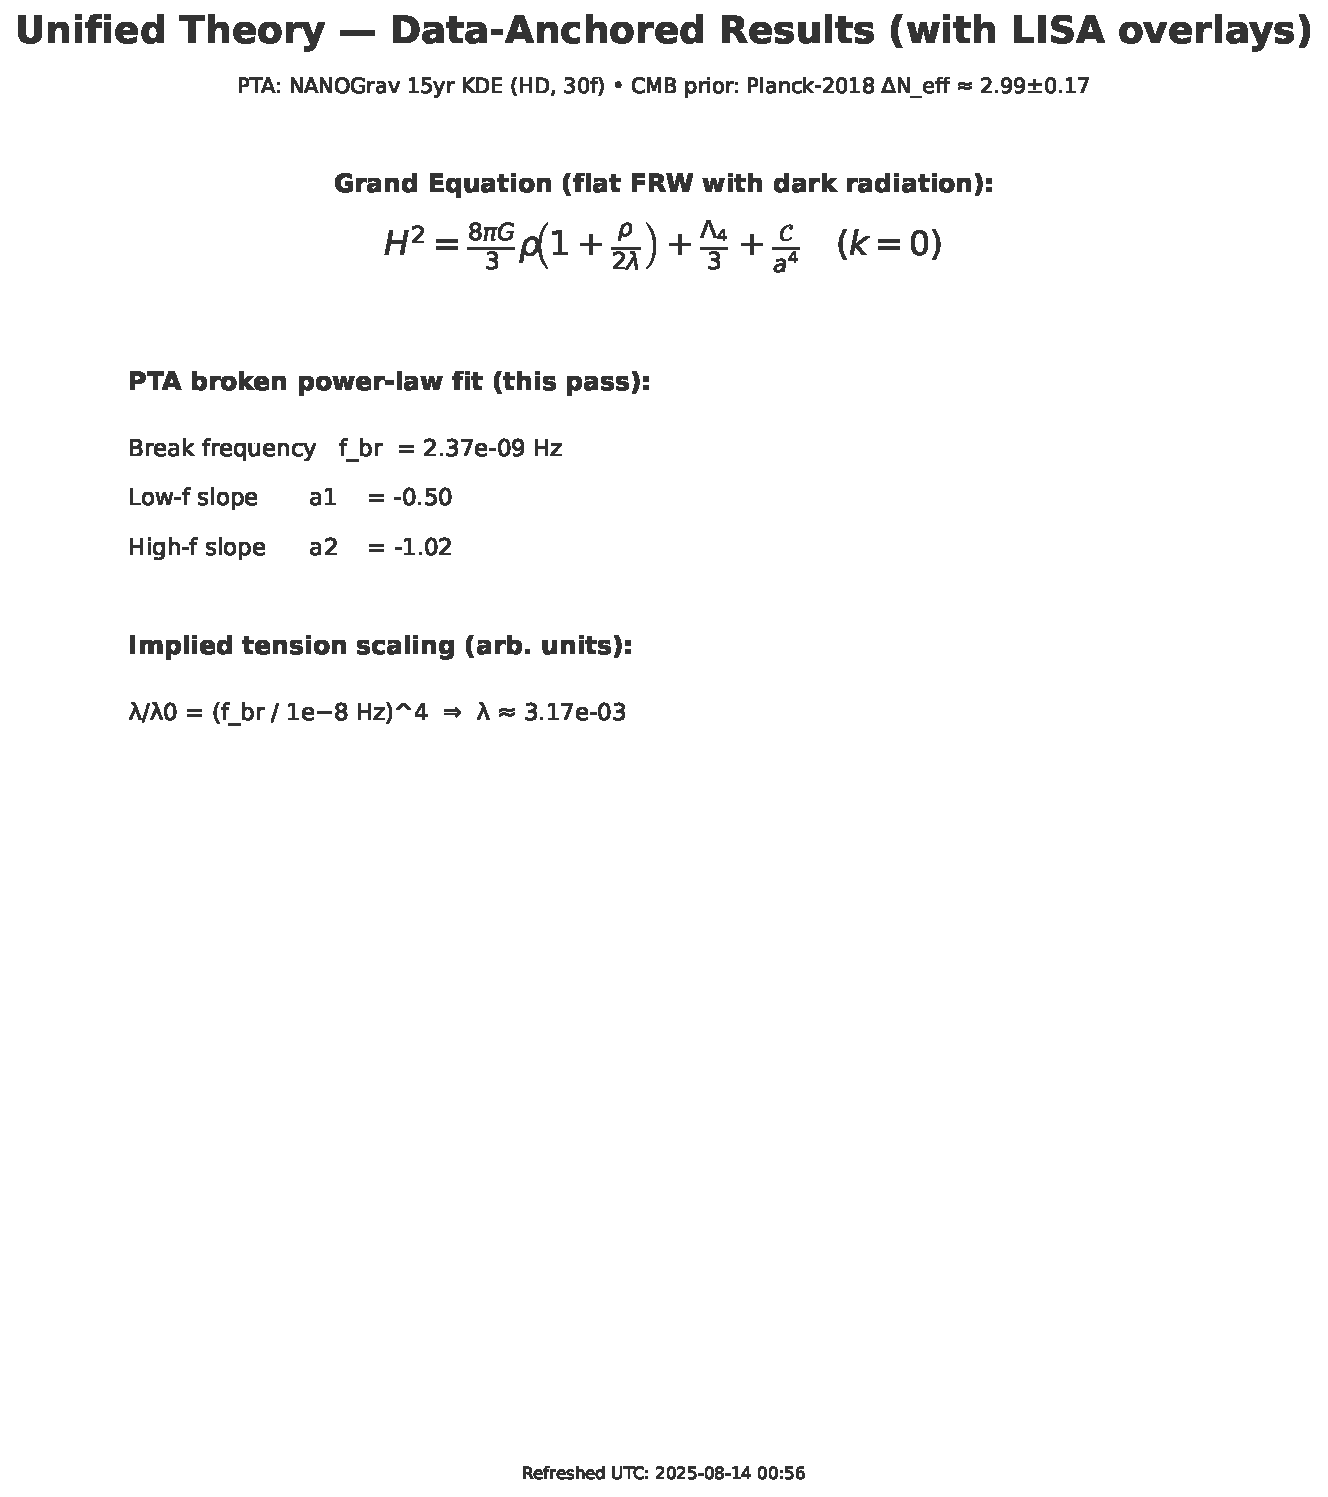
\includegraphics[width=\linewidth]{figs/Results_TwoPager_REALDATA_LISA_OVERLAYS_20250814_005546.pdf}
\caption{PTA fit with illustrative LISA overlays (4-yr vs 10-yr). Y-axes differ in units.}
\end{figure}
\end{document}
